\subsection{Schéma de la database}

Database : \\

\begin{figure}[h]
	\centering
	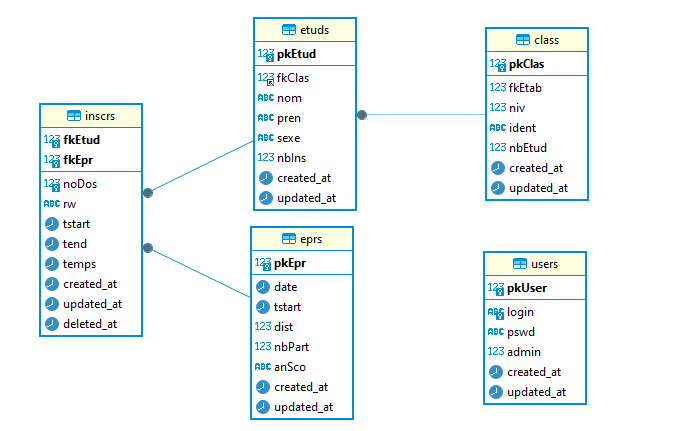
\includegraphics[width=15cm]{images/Database}
	\caption{Schéma de la database du projet}
\end{figure}

\begin{itemize}[label=$\bullet$]
	\item Par rapport à l'ébauche de schéma relationnel de la DB de départ, quelque modifications ont été apportées :
	\begin{itemize}[label=$\bullet$]
		\item Ajout des colonnes created\_at et updated\_at ; attributs généré par défaut par laravel que j'ai choisi de laisser, si jamais nous décidions des triers des informations sur leur date de création et/ou de mise à jour
		\item Suppresion de la clé primaire PkInscr de la table Inscrs : J'ai choisi d'utilisé une clé primaire composite de [fkEtud;fkEpr] afin de mieux controler la duplication de données dans cette table
	\end{itemize}
\end{itemize}